\documentclass[a4paper, 12pt]{article}

\usepackage{cmap}
\usepackage{mathtext} 
\usepackage[T2A]{fontenc}
\usepackage[utf8]{inputenc}
\usepackage[english,russian]{babel}	

\usepackage{amsfonts,amssymb,amsthm,mathtools}
\usepackage{amsmath}
\usepackage{icomma} 

\usepackage{graphicx} 
\graphicspath{{Picturies/}, {Picturies/air/}, {Picturies/co2/}, {Picturies/work2_/}}
\usepackage{wrapfig}

\usepackage{array,tabularx,tabulary,booktabs}
\usepackage{longtable}
\usepackage{multirow}

\usepackage{caption}
\captionsetup{labelsep=period}

\renewcommand{\phi}{\varphi}
\newcommand{\eps}{\varepsilon}
\newcommand{\parag}[1]{\paragraph*{#1:}}

\newcounter{Points}
\setcounter{Points}{1}
\newcommand{\point}{\arabic{Points}. \addtocounter{Points}{1}}

\author{Вязовцев Андрей, Б01-005}
\date{16.03.21}
\title{Лабораторная работа 2.1.3. Определение теплоты испарения жидкости}

\begin{document}

\maketitle

\parag {Цель работы}
1) измерение частоты колебаний и длины волны при резонансе звуковых колебаний в газе, заполняющем трубу; 2) определение показателя адиабаты с помощью уравнения состояния идеального газа.

\parag {В работе используются}
звуковой генератор (ГЗ); электронный осциллограф (ЭО); микрофон; телефон; раздвижная труба; теплоизолированная труба, обогреваемая водой из термостата; баллон со сжатым углекислым газом; газгольдер.

\parag {Теоритическая справка} ~\\

Распространение звука в газе является адиабатическим процессом, поэтому его скорость зависит от показателя адиабаты $\gamma$. Выражается она следующей формулой:

\[
    c = \sqrt{\gamma ~\frac{RT}{\mu}}
\]

Отсюда находим:

\[
    \gamma = \frac{\mu}{RT}c^2
\]

Т.~к. в запаянном сосуде волны, распространяющиеся вдоль трубы, испытывают отражения, резонанс будет наблюдаться, если длина трубы $L$ удовлетворяет следующему условию:

\[
    L = n \frac{\lambda}{2},~n \in \mathbb{Z} 
\]

При этом будут места, где слои газа не испытывают смещения (узлы смещения), они повторяются по всей длине через $\displaystyle \frac{\lambda}{2}$. Между ними находятся максимумы смещения (пучности).

Скорость звука так связана с его частотой $f$ и длиной волны $\lambda$:

\begin{equation} \label{eq:main}
    c = \lambda f
\end{equation}

Подбор условий, при которых возникает резонанс, можно производить двояко:

1. Изменение длины трубы. Для последовательных резонансов имеем:

\[
    L_n = n \frac{\lambda}{2},~L_{n+1} = (n+1) \frac{\lambda}{2}, ~\dots, ~ L_{n+k} = n\frac{\lambda}{2} + k \frac{\lambda}{2}
\]

Отсюда следует, что $L (k)$ --- линейная зависимость, а коэффициент наклона данной прямой есть $\displaystyle \frac{\lambda}{2}$.

2. Изменение частоты звуковых колебаний. Для последовательных резонансов получим:

\begin{equation} \label{eq:case2}
    L = \frac{\lambda_1}{2} n = \frac{\lambda_2}{2} (n + 1) = ~ \dots ~ = \frac{\lambda_k}{2} (n + k)
\end{equation}

Из уравнений \eqref{eq:main} и \eqref{eq:case2} получаем:

\[
    f_{k+1} = f_1 + \frac{c}{2L}k
\]

Следовательно, $f (k)$ --- линейная зависимость, её коэффициент наклона --- $\displaystyle \frac{c}{2L}$

\parag {Экспериментальная установка} ~

\begin{figure}[!h]
    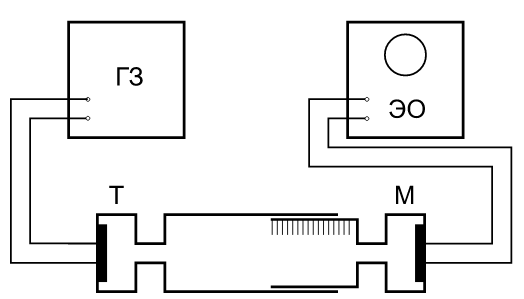
\includegraphics[scale = 0.4]{Workplace1}
    \caption{Установка для измерения скорости звука \\ при помощи раздвижной трубы} \label{work:1}
\end{figure}

\begin{figure}[!h]
    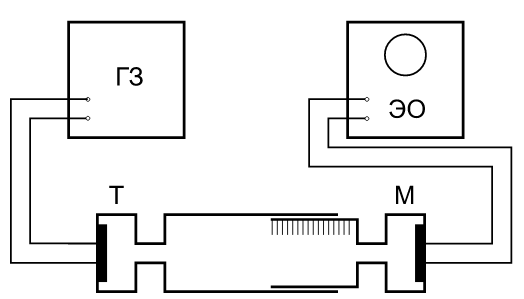
\includegraphics[scale = 0.4]{Workplace1}
    \caption{Установка для изучения зависимости \\ скорости звука от температуры} \label{work:2}
\end{figure}

\parag {Ход работы} ~\\

\point Сначала проведём эксперименты на экпериментальной установке №\ref{work:1}. Включим в ЭО и ГЗ, подождём, пока они прогреются (5-7 минут). После этого настроим осциллограф. Продуем трубу от углекислого газа, который мог остаться от предыдущих опытов.

\point Рассчитаем, в каком диапозоне частот следует вести  измерения, чтобы можно было наблюдать 2-5 резонансов. Т.~к. изначально труба имеет длину $L_{min} = 700 \pm 5 \text {мм}$ и может удлиняться до $L_{min} = 930 \pm 5 \text {мм}$, из несложных соображений получаем:

\begin{align*}
    f_{min} = \frac{(2-1)c}{2(L_{max} - L_{min})} \approx 700 ~\text{Гц} \\
    f_{max} = \frac{(5-1)c}{2(L_{max} - L_{min})} \approx 3 ~\text{кГц}
\end{align*}

Стоит отметить, что т.~к. скорость звука несколько выше, а в результате экспериментов мы будем получать больше 5 резонансов, измерения будут проводиться в немного другом диапозоне частот.

\point Будем плавно уменьшать длину трубы от $L_{max}$ до $L_{min}$ и фиксировать, при каких длинах трубы $L$ наблюдается резонанс. Проведём данные измерения для 6 различных частот. Результаты внесём в табл. \ref{tabl:1}.

\begin{table}[!h]
    \begin{tabularx}{\linewidth}{|c|X|X|X|X|X|X|X|X|}
        \hline
        $f$, кГц & \multicolumn{8}{c|}{$L$, мм} \\ \hline
        $2,0$ & $17,8$ & $10,0$ & $2,0$ &\multicolumn{5}{c|}{}\\ \hline
        $2,5$ & $21,6$ & $15,2$ & $8,6$ & $2,0$ & \multicolumn{4}{c|}{} \\ \hline
        $3,0$ & $21,6$ & $16,2$ & $10,9$ & $5,5$ & $0,0$ & \multicolumn{3}{c|}{} \\ \hline
        $3,5$ & $20,0$ & $15,2$ & $10,5$ & $5,7$ & $1,0$ & \multicolumn{3}{c|}{}\\ \hline
        $4,2$ & $22,7$ & $19,1$ & $15,6$ & $12,1$ & $8,5$ & $4,9$ & $1,3$ & \\ \hline
        $5,0$ & $22,2$ & $19,1$ & $16,1$ & $13,0$ & $10,0$ & $6,9$ & $3,8$ & $0,7$ \\ \hline 
    \end{tabularx}
\caption{Резонансы воздуха, установка 1}
\label{tabl:1}
\end{table}

\point Изобразим зависимость $\Delta L (k)$ для каждого значения частоты, где $\Delta L = L_{n+k} - L_n$. 

\begin{tabular}{cc}
    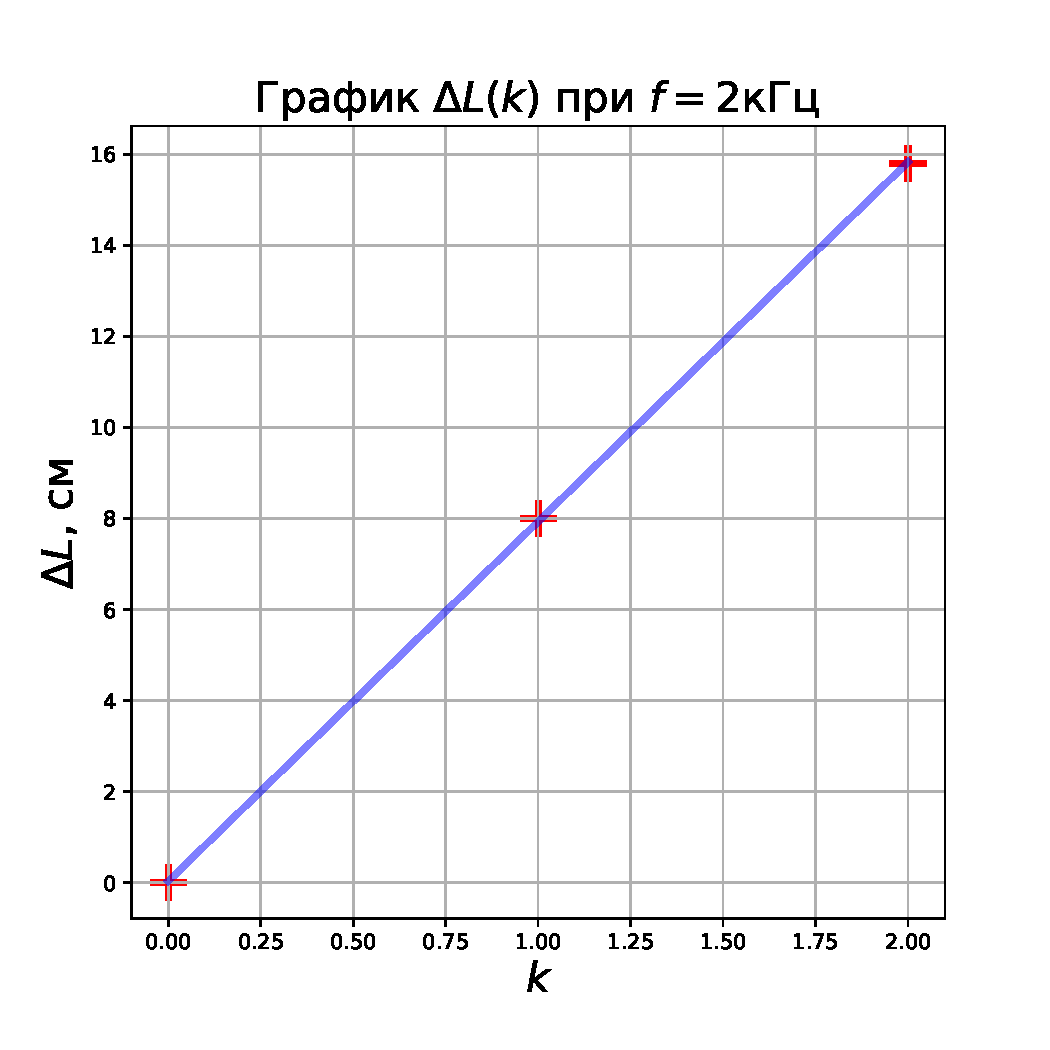
\includegraphics[scale = 0.4]{air0} &
    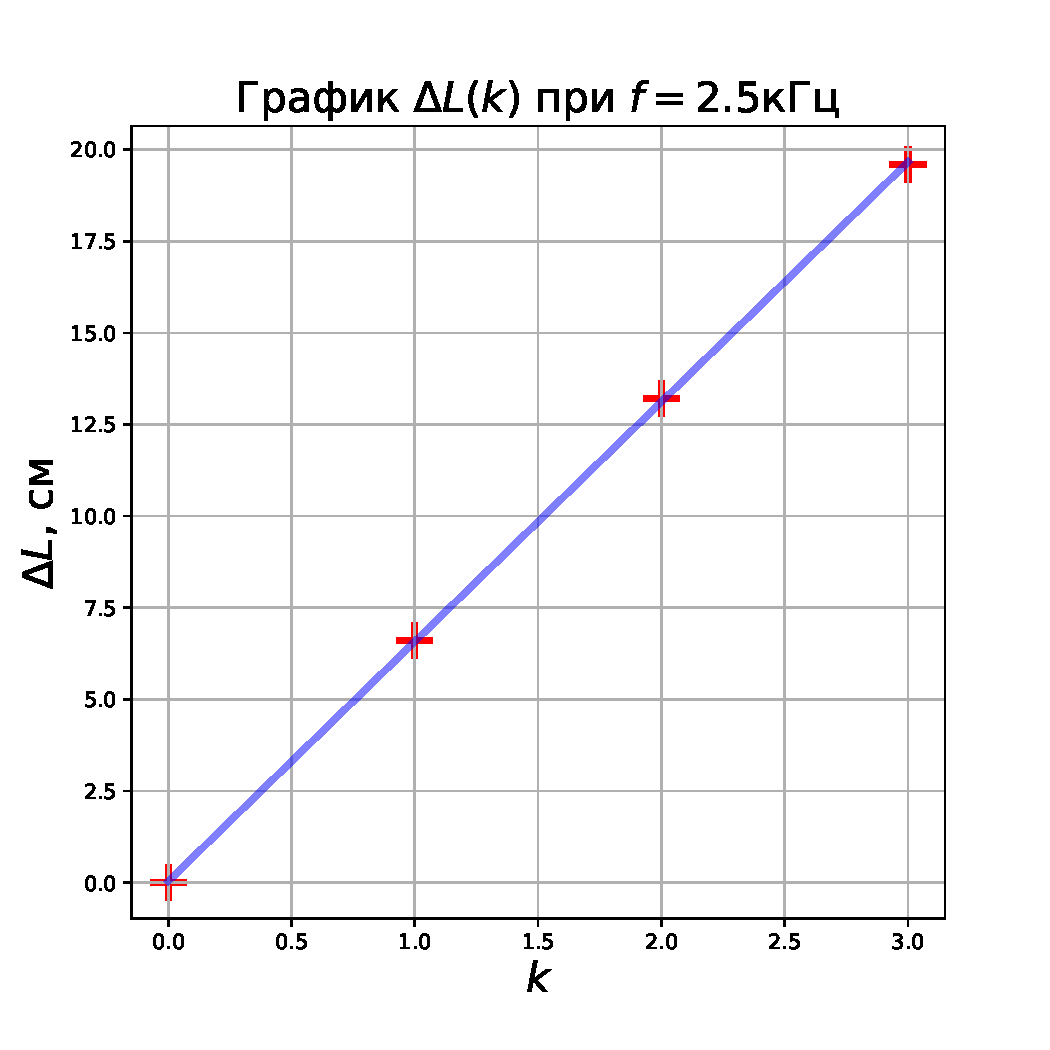
\includegraphics[scale = 0.4]{air1} \\
    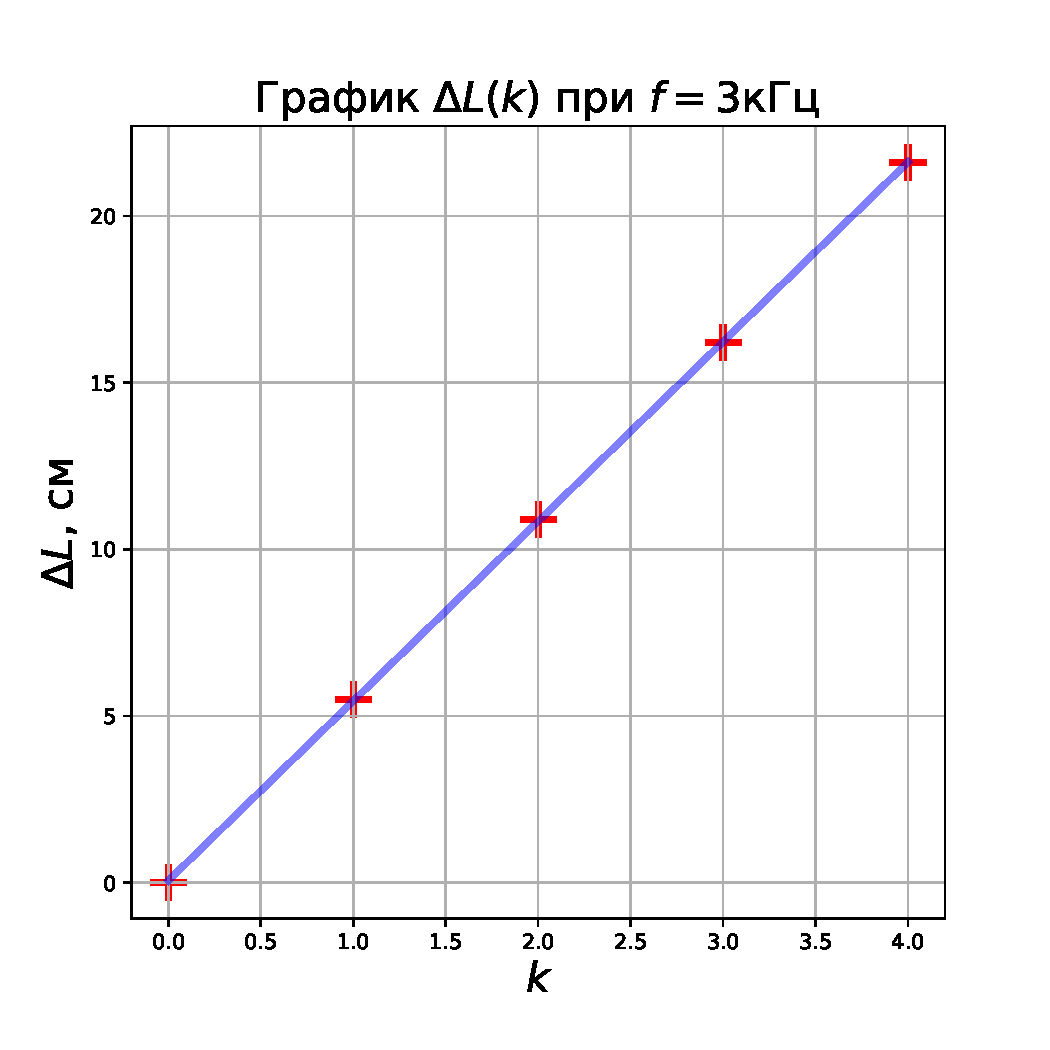
\includegraphics[scale = 0.4]{air2} &
    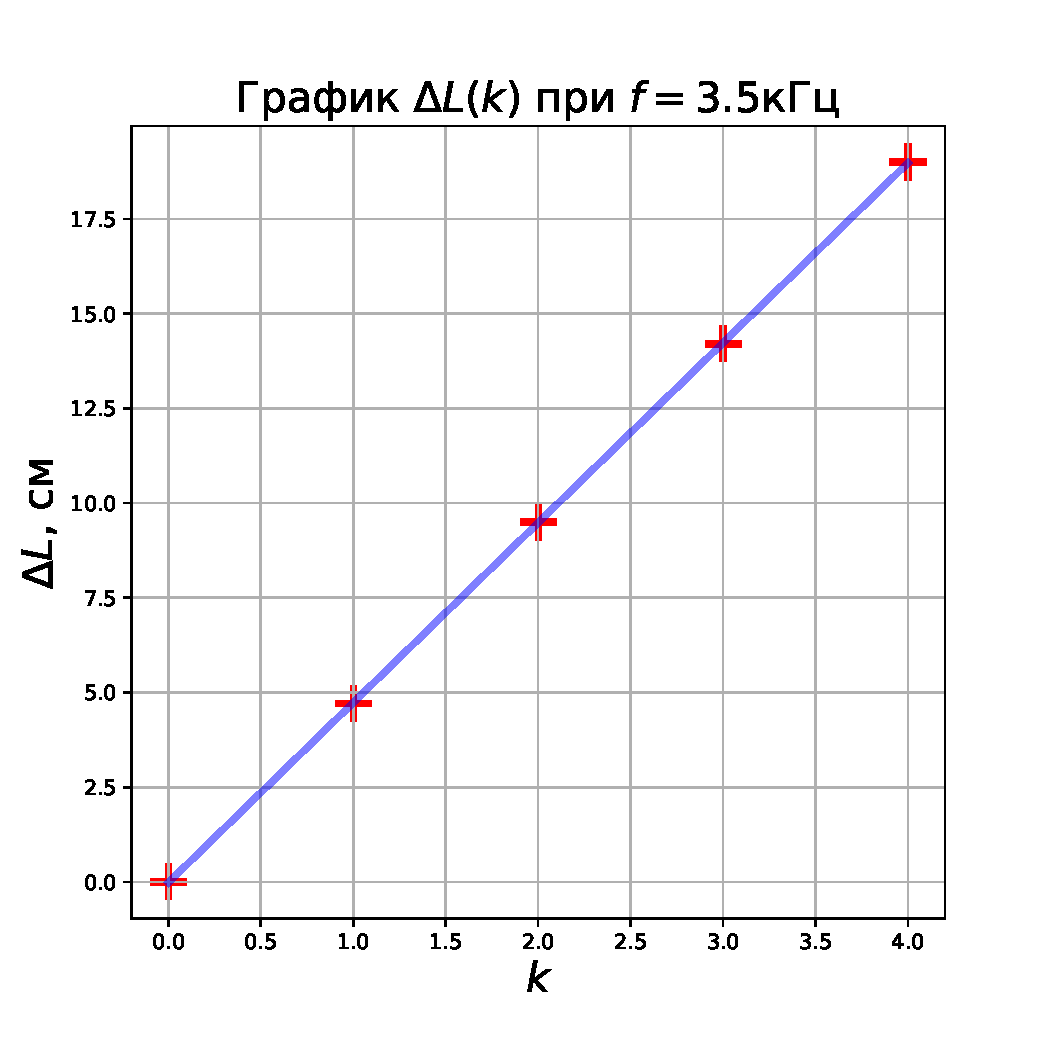
\includegraphics[scale = 0.4]{air3} \\
\end{tabular}

\begin{tabular}{cc}
    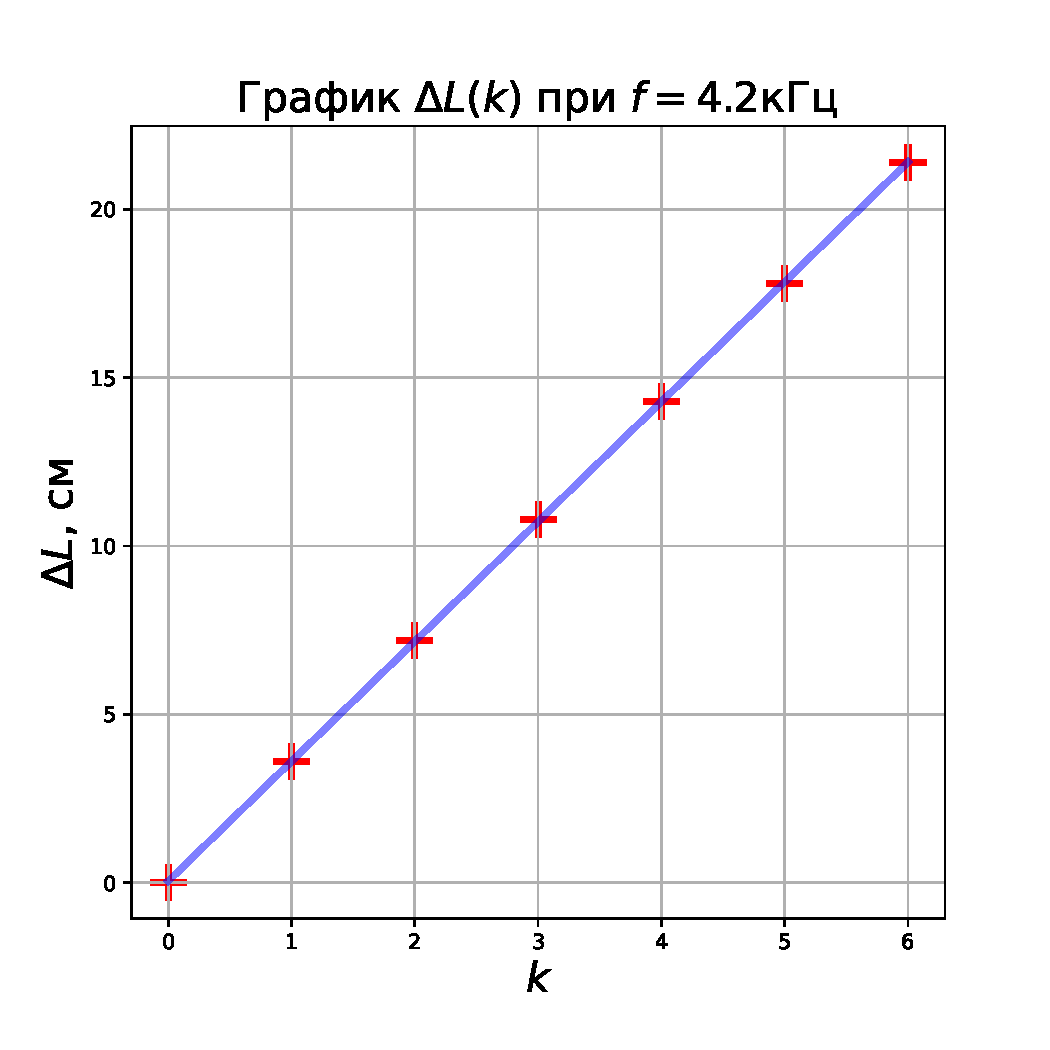
\includegraphics[scale = 0.4]{air4} &
    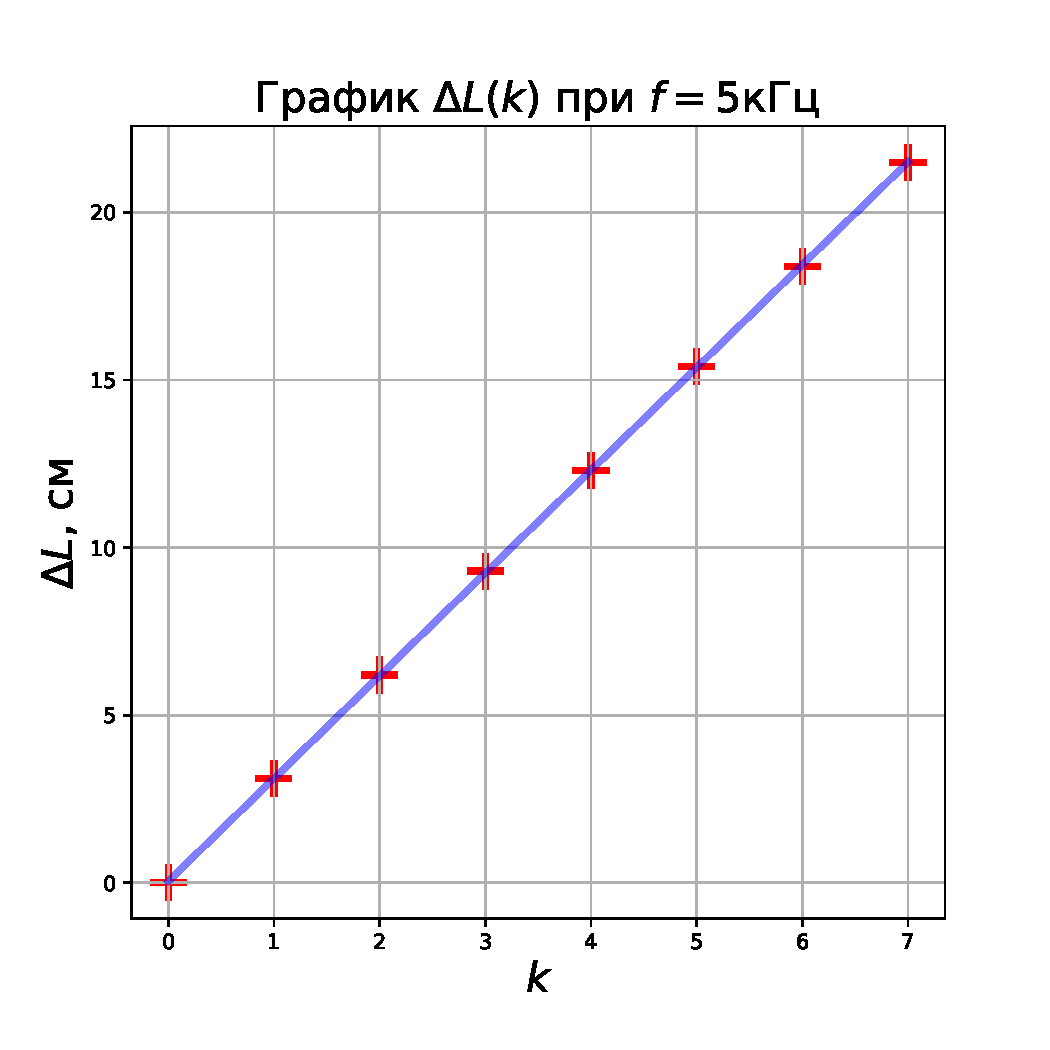
\includegraphics[scale = 0.4]{air5}
\end{tabular}

\point Теперь найдём $\displaystyle \frac{\lambda}{2}$ как коэффициент наклона этих графиков, а после можно найти скорость звука:

\begin{align*}
    c_{2.0} &= 316 ~\frac{\text{м}}{\text{с}^2} &
    c_{2.5} &= 327 ~\frac{\text{м}}{\text{с}^2} &
    c_{3.0} &= 323 ~\frac{\text{м}}{\text{с}^2} \\
    c_{3.5} &= 333 ~\frac{\text{м}}{\text{с}^2} &
    c_{4.2} &= 299 ~\frac{\text{м}}{\text{с}^2} &
    c_{5.0} &= 307 ~\frac{\text{м}}{\text{с}^2} 
\end{align*}

Т.~к. погрешность генератора частот пренебрежимо мала ($\eps_f \approx 0,01\%$), верно следующее: $\displaystyle \eps_c = \eps_\lambda$. Из формулы для погрешности МНК получаем:

\begin{align*}
    \eps_{c_{2.0}} &= 0,4\% &
    \eps_{c_{2.5}} &= 0,4\% &
    \eps_{c_{3.0}} &= 0,3\% \\
    \eps_{c_{3.5}} &= 0,2\% &
    \eps_{c_{4.2}} &= 0,2\% &
    \eps_{c_{5.0}} &= 0,2\% 
\end{align*}

Таким образом, наиболее точными измерениями являются последние, в которых было больше резонансов. Стоит отметить, что значения, полученные в различных опытах, отличаются не более чем на 10\%. Значит, эти значения находятся в согласии друг с другом.

\point Продуем трубу углекислым газом, после чего найдём скорость звука в углекислом газе, для этого проделаем те же действия, что и в предыдущих пунктах. Внесём результаты экспериментов в табл. \ref{tabl:2}, построим графики, найдём $c$ и погрешности.

\begin{table}[!h]
    \begin{tabularx}{\linewidth}{|c|X|X|X|X|X|X|X|}
        \hline
        $f$, кГц & \multicolumn{7}{c|}{$L$, мм} \\ \hline
        $2,0$ & $22,4$ & $15,7$ & $9,1$  & $2,7$ & \multicolumn{3}{c|}{} \\ \hline
        $2,5$ & $17,9$ & $12,0$ & $6,0$  & $0,4$ & \multicolumn{3}{c|}{} \\ \hline
        $3,0$ & $21,9$ & $16,8$ & $11,8$ & $7,0$ & $2,2$ & \multicolumn{2}{c|}{} \\ \hline
        $3,5$ & $19,9$ & $15,8$ & $11,5$ & $7,4$ & $3,5$ & \multicolumn{2}{c|}{} \\ \hline
        $4,0$ & $22,7$ & $18,8$ & $15,2$ & $11,6$ & $8,2$ & $4,5$ & $1,0$ \\ \hline 
    \end{tabularx}
\caption{Резонансы углекислого газа, установка 1}
\label{tabl:2}
\end{table}

\begin{tabular}{cc}
    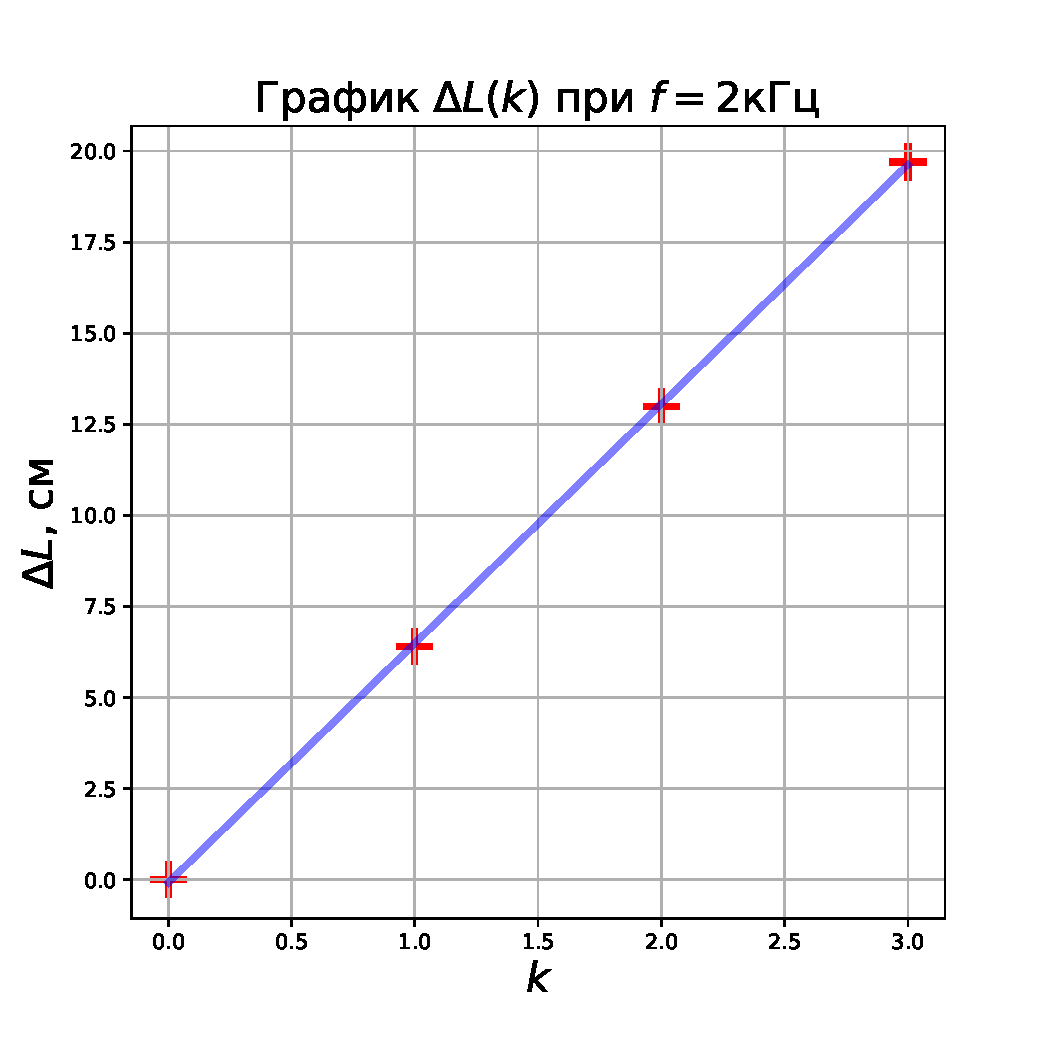
\includegraphics[scale = 0.4]{co20} &
    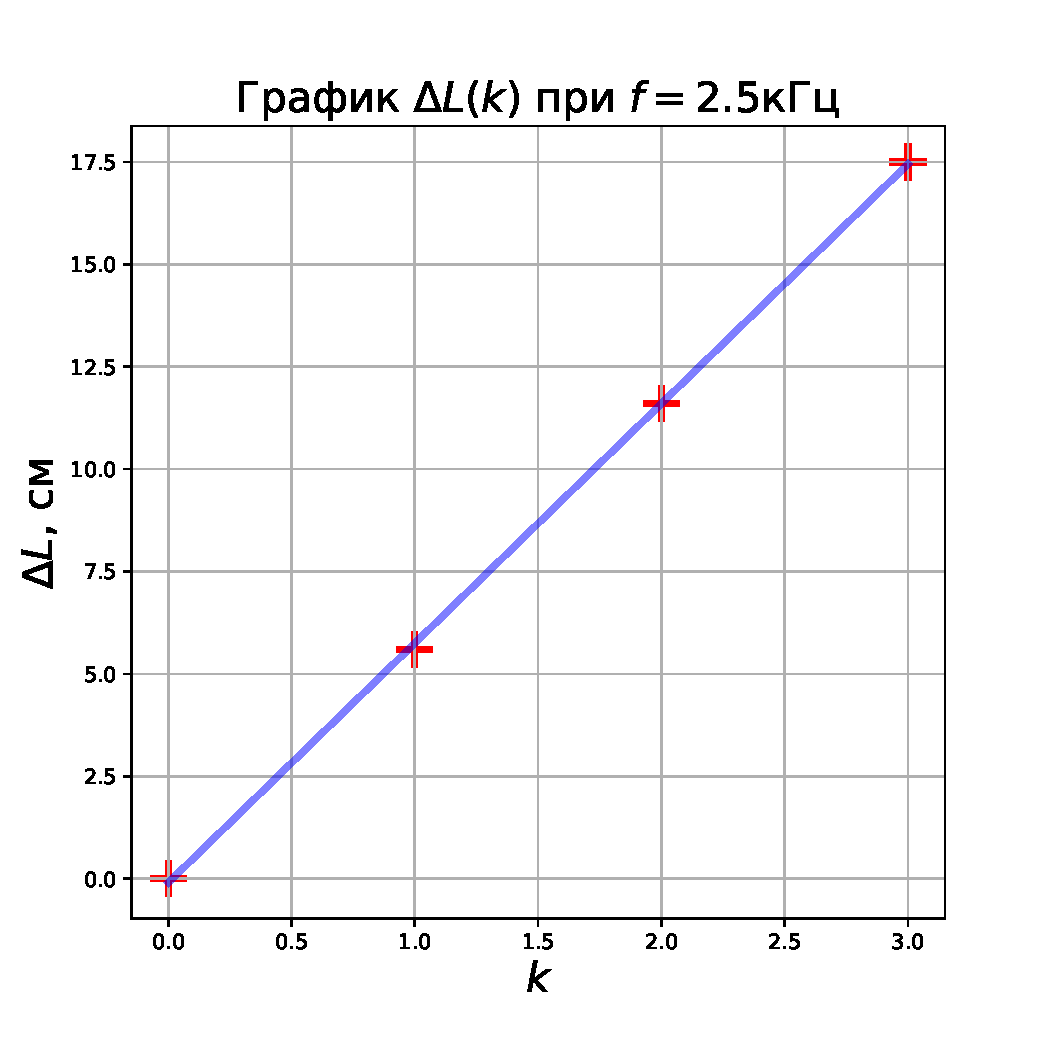
\includegraphics[scale = 0.4]{co21} \\
    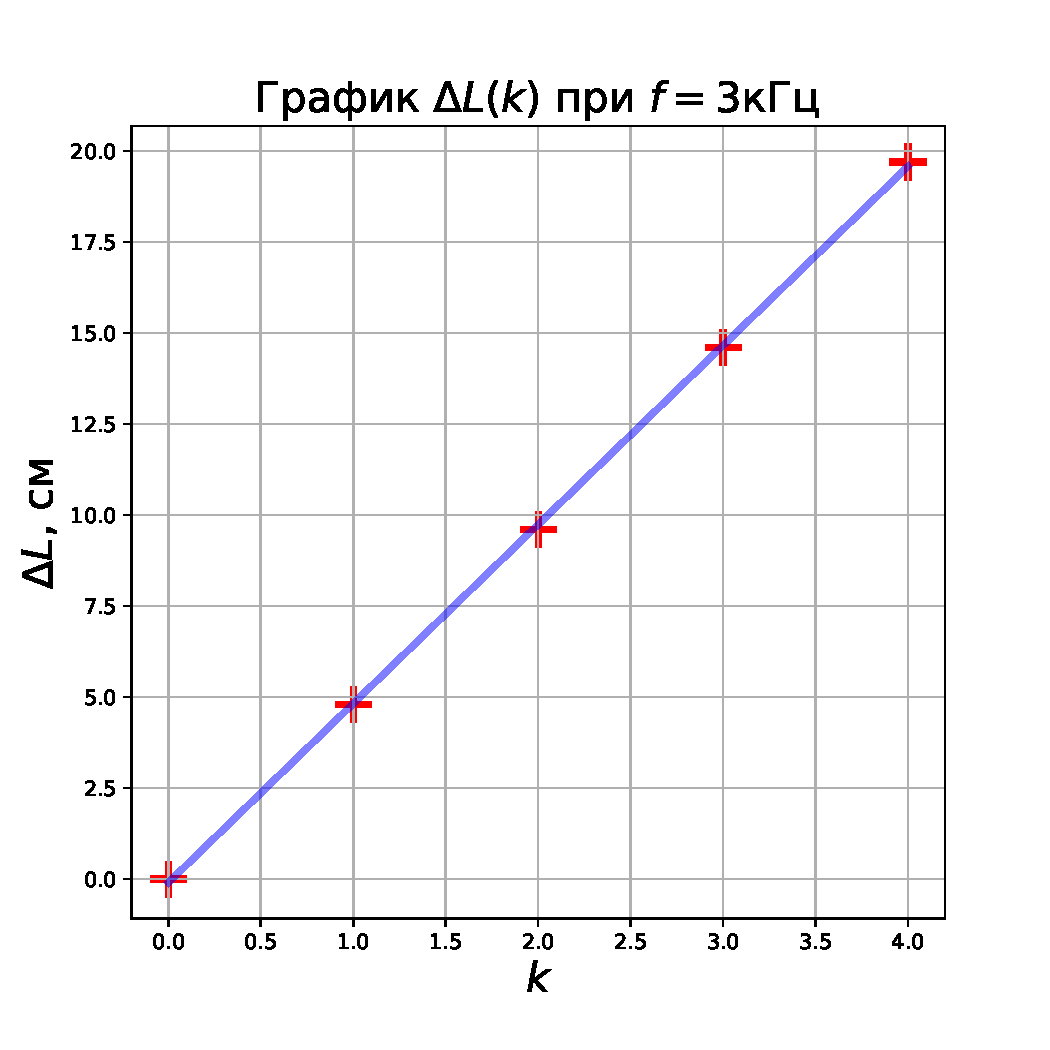
\includegraphics[scale = 0.4]{co22} &
    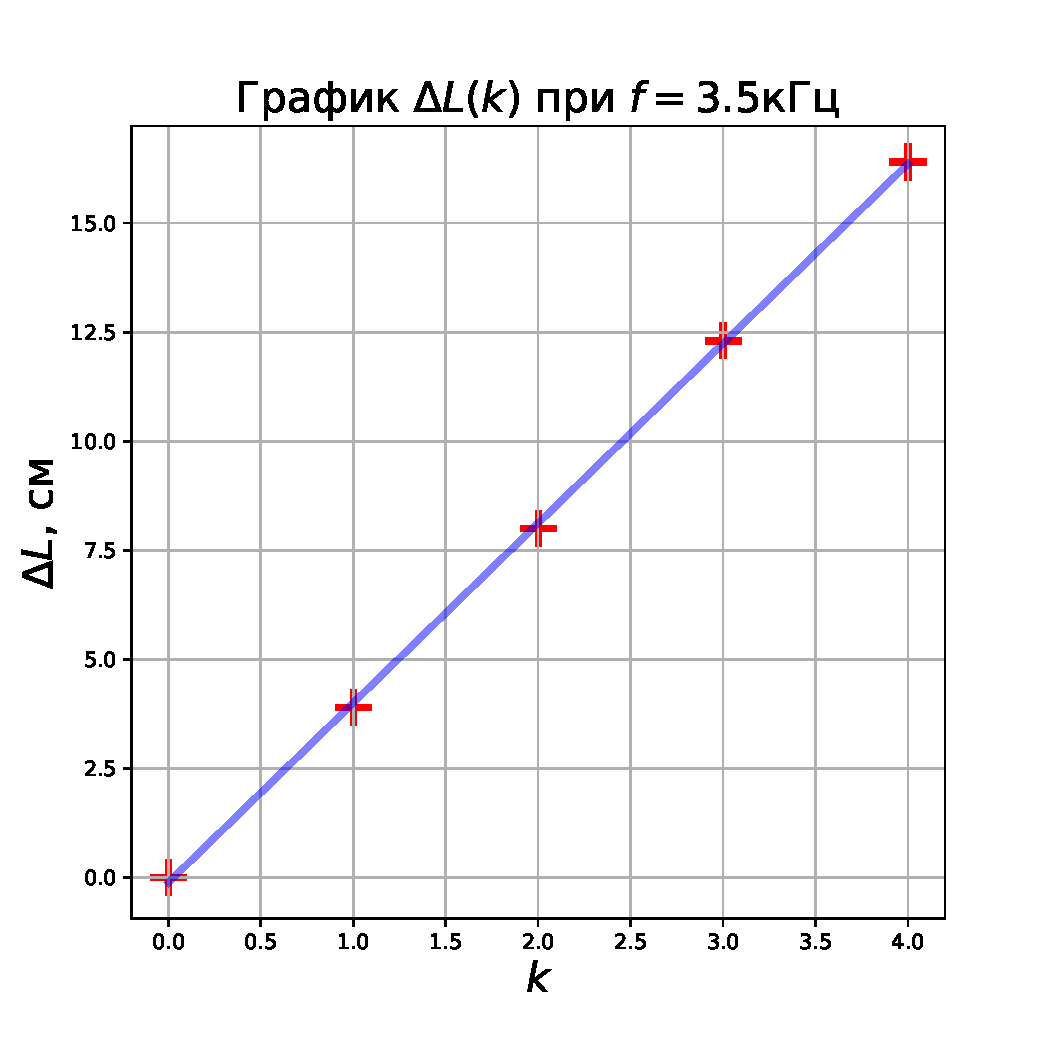
\includegraphics[scale = 0.4]{co23} \\
\end{tabular}

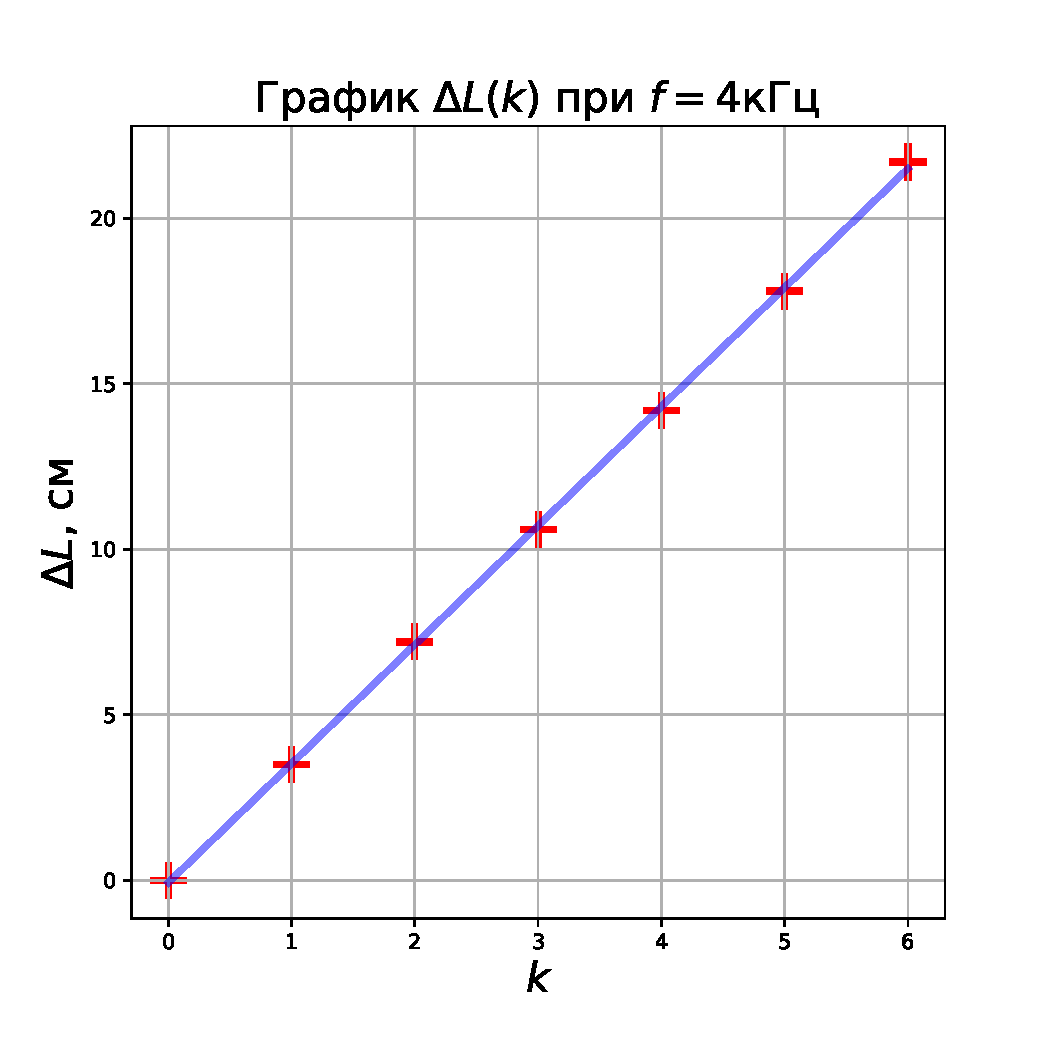
\includegraphics[scale = 0.4]{co24}

Скорости звука:

\begin{align*}
    c_{2.0} &= 263 ~\frac{\text{м}}{\text{с}^2} &
    c_{2.5} &= 293 ~\frac{\text{м}}{\text{с}^2} &
    c_{3.0} &= 295 ~\frac{\text{м}}{\text{с}^2} \\
    c_{3.5} &= 288 ~\frac{\text{м}}{\text{с}^2} &
    c_{4.2} &= 288 ~\frac{\text{м}}{\text{с}^2}  
\end{align*}

Их погрешности:

\begin{align*}
    \eps_{c_{2.0}} &= 0,5\% &
    \eps_{c_{2.5}} &= 0,7\% &
    \eps_{c_{3.0}} &= 0,6\% \\
    \eps_{c_{3.5}} &= 0,7\% &
    \eps_{c_{4.2}} &= 0,6\% 
\end{align*}

\point Теперь проведём измерения на второй установке. Будем изменять частоту ГЗ, и фиксировать последовательные резонансы. Сделаем это для нескольких температур. Результаты занесём в табл. \ref{tabl:3}.

\begin{table}[!h]
    \begin{tabularx}{\linewidth}{|c|X|X|X|X|X|}
        \hline
        $t$, $^o C$ & \multicolumn{5}{c|}{$f$, Гц} \\ \hline
        $23$ & $195$ & $450$ & $660$ & $870$ & $1100$ \\ \hline
        $30$ & $220$ & $460$ & $660$ & $880$ & $1110$ \\ \hline
        $40$ & $207$ & $465$ & $675$ & $895$ & $1115$ \\ \hline
        $50$ & $205$ & $470$ & $690$ & $910$ & $1135$ \\ \hline
        $60$ & $203$ & $472$ & $695$ & $922$ & $1150$ \\ \hline 
    \end{tabularx}
\caption{Резонансы, установка 2}
\label{tabl:3}
\end{table}

Графики $f (k)$:

\begin{tabular}{cc}
    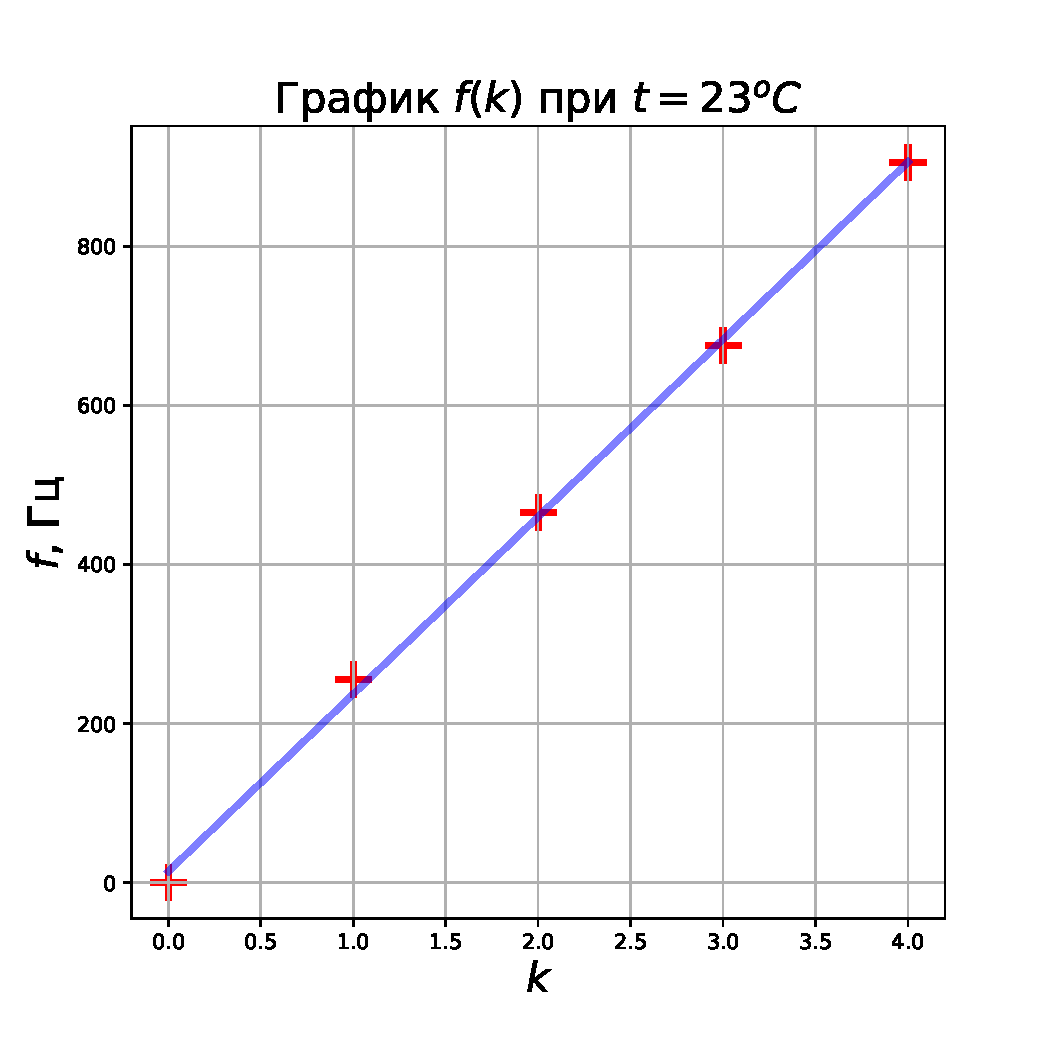
\includegraphics[scale = 0.4]{work2_0} &
    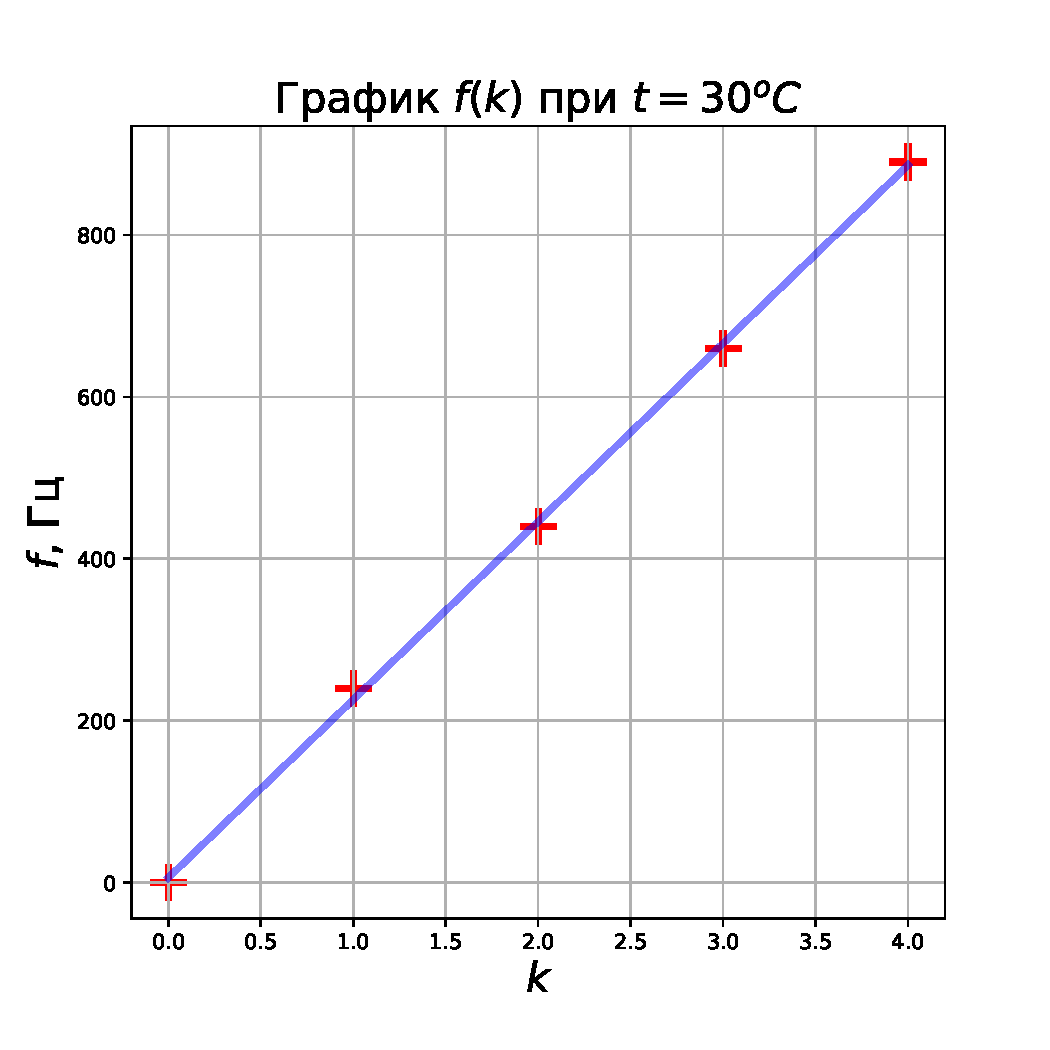
\includegraphics[scale = 0.4]{work2_1} \\
    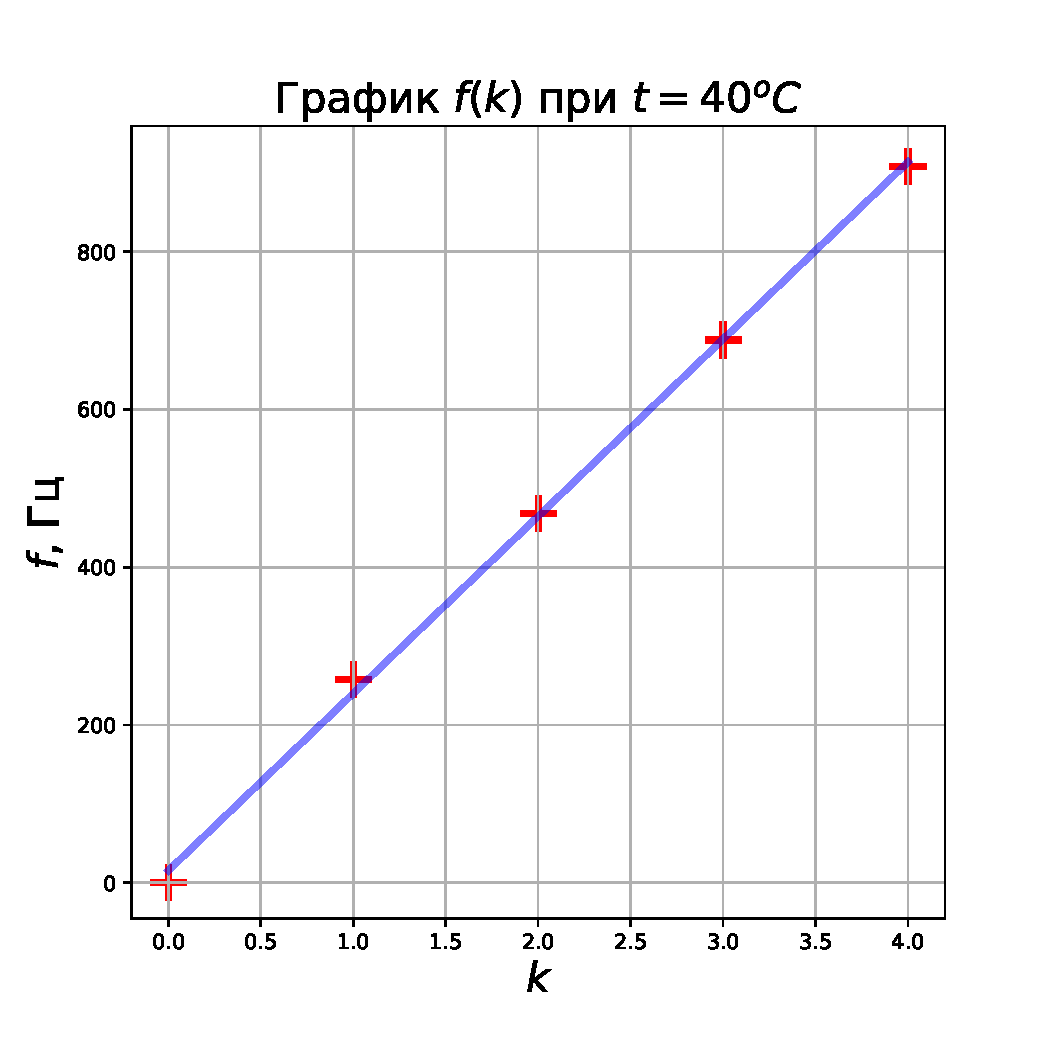
\includegraphics[scale = 0.4]{work2_2} &
    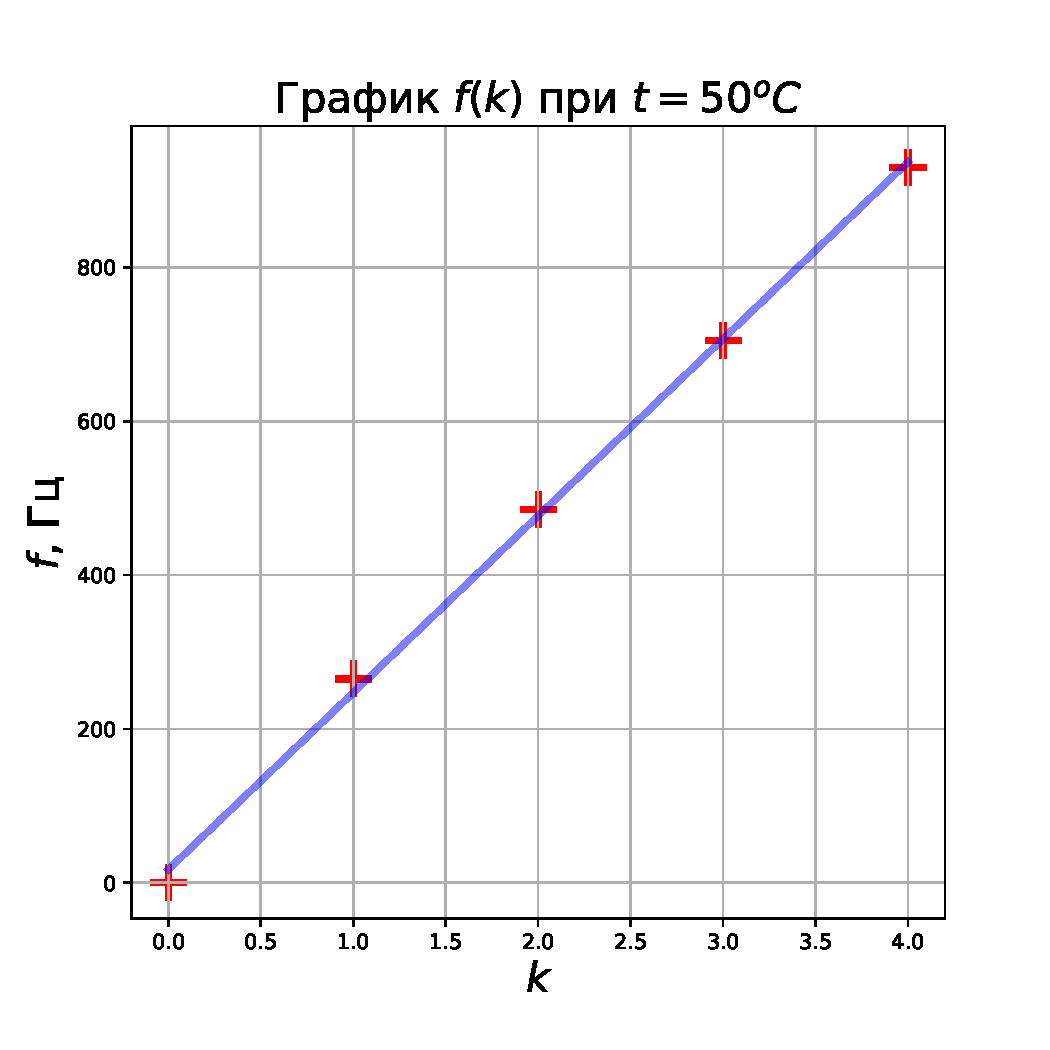
\includegraphics[scale = 0.4]{work2_3} \\
    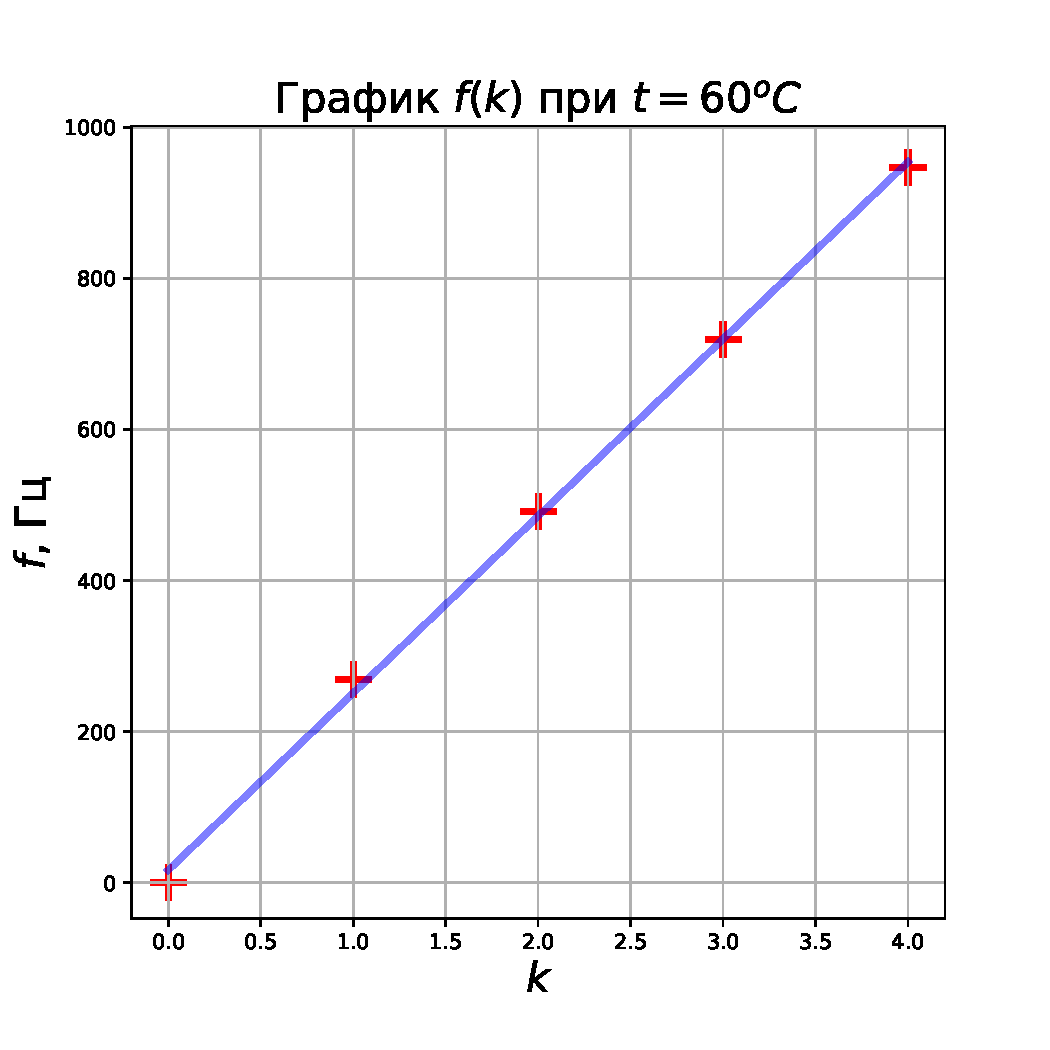
\includegraphics[scale = 0.4]{work2_4} 
\end{tabular}

По коэффициенту наклона, который равен $\displaystyle \frac{c}{2L}$ найдём скорость звука. Учтём, что $L = 700$ мм.

\begin{align*}
    c_{23} &= 312 ~\frac{\text{м}}{\text{с}^2} &
    c_{30} &= 308 ~\frac{\text{м}}{\text{с}^2} &
    c_{40} &= 314 ~\frac{\text{м}}{\text{с}^2} \\
    c_{50} &= 322 ~\frac{\text{м}}{\text{с}^2} &
    c_{60} &= 328 ~\frac{\text{м}}{\text{с}^2}  
\end{align*}

По аналогии с установкой 1 находим погрешности для скорости звука:

\begin{align*}
    \eps_{c_{23}} &= 1,5\% &
    \eps_{c_{30}} &= 1,1\% &
    \eps_{c_{40}} &= 1,6\% \\
    \eps_{c_{50}} &= 1,7\% &
    \eps_{c_{60}} &= 1,6\% 
\end{align*}

\point Найдём показатель адиабаты по формуле:

\[
    \gamma = \frac{\mu}{RT}c^2 \approx \frac{29 \cdot 10^{-3}}{8.314 \cdot 296} \cdot 308^2 \approx 1,11
\]

Для нахождения относительной погрешности воспользуемся тем, что $\displaystyle \eps_{T} = \frac{1}{296}$, a $\eps_c = \eps_{c_{23}} = 1,5\%$

\[
    \eps_\gamma = \sqrt{\eps_c^2 + \eps_T^2} \approx 1,5\%
\]

Итак, $\gamma = 1,11 \pm 0,02$

\end{document}
